\documentclass[11pt]{article}
\usepackage[margin=1in]{geometry}
\usepackage{amsmath,amssymb}
\usepackage{enumitem}
\usepackage{graphicx}
\usepackage{xcolor}
\usepackage{tcolorbox}
\tcbuselibrary{breakable,skins}
\usepackage{parskip}
\usepackage{hyperref}
\hypersetup{colorlinks=true, urlcolor=blue, linkcolor=blue}

\newcommand{\E}{\mathbb{E}}
\newcommand{\hM}{\hat{M}}
\newcommand{\hlam}{\hat{\lambda}}
\newcommand{\Nsub}{N_{\mathrm{sub}}}
\newcommand{\Uobs}{U_{\mathrm{obs}}}

\title{\vspace{-2em}\textbf{Library complexity via subsampling}\\[0.3em]\large
A primer for Q2(a)\\[0.6em]
\normalsize \textit{Supplementary material to Computational Genomics, Exercise 2 (Library Complexity)}}
\author{Roee Tekoah \\ \texttt{roee.tekoah@mail.huji.ac.il}}
\date{}

\begin{document}
\maketitle
\vspace{-1em}

\section{The question}

We are handed a sequencing run summarised as a list of fragments and per-fragment read
counts: $(\mathrm{chr}_j, \mathrm{start}_j, \mathrm{end}_j, n_j)$ for $j = 1, \dots, U$,
where $U$ is the number of distinct fragments observed and $N = \sum_j n_j$ is the total
number of reads. We want to estimate the \textbf{true library complexity} $M$, i.e.\ the
number of distinct molecules that were in the library before sequencing began, including
the ones we never saw because they happened to receive zero reads.

The point of the subsampling procedure (and the alternative to it from Q1) is that we
\emph{don't} just want a one-shot estimate of $M$ from the single observed pair $(N, U)$
-- we want to use the \emph{shape} of how unique fragments accumulate as a function of
sequencing depth.

\section{The model and the saturation curve}

Under the working assumptions of Q1 (every original molecule has a unique sequence;
per-molecule read counts are i.i.d.\ $\mathrm{Poisson}(\lambda)$ with $\lambda = N/M$
in the uniform-sampling case), a textbook calculation gives the expected number of
unique observed fragments as a function of $N$:
\begin{equation}
   \E[U \mid N] \;=\; M\bigl(1 - e^{-N/M}\bigr).
   \label{eq:saturation}
\end{equation}

This is the \textbf{library saturation curve}. It is worth absorbing what it says:

\begin{itemize}[leftmargin=2em,itemsep=2pt]
  \item \textbf{Cap at $M$.} As $N \to \infty$, $e^{-N/M} \to 0$, so $\E[U] \to M$. No
        matter how deeply we sequence, the number of distinct fragments we can ever see
        is bounded by the library complexity.
  \item \textbf{Linear at low depth.} For small $N$ (specifically $N \ll M$),
        $1 - e^{-N/M} \approx N/M$, so $\E[U] \approx N$: every additional read hits a
        fresh fragment, because the chance of accidentally hitting one we've already
        seen is tiny.
  \item \textbf{The exponential interpolates.} The factor $e^{-N/M}$ is precisely the
        Poisson probability that a given fragment receives zero reads under expected
        coverage $\lambda = N/M$, and it interpolates smoothly between the linear
        regime and the saturation cap. At the symbolic point $N = M$, we have
        $\E[U] = M(1 - e^{-1}) \approx 0.63\,M$ -- already past the linear regime, not
        yet saturated.
\end{itemize}

\begin{figure}[h]
\centering
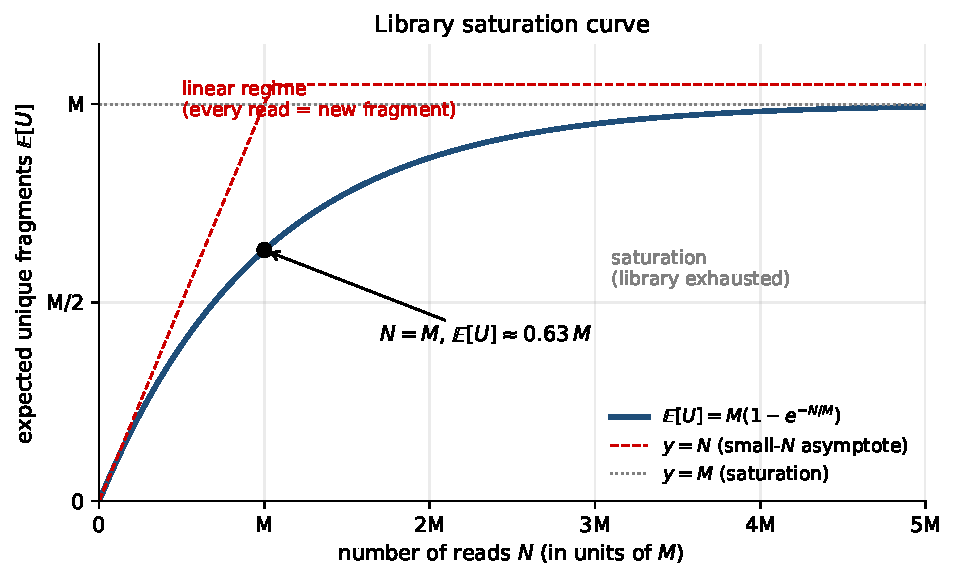
\includegraphics[width=0.8\linewidth]{fig1_saturation.pdf}
\caption{The library saturation curve $\E[U] = M(1-e^{-N/M})$. Linear for $N \ll M$,
plateaus at $M$ for $N \gg M$, hits $0.63\,M$ at $N = M$.}
\label{fig:sat}
\end{figure}

\section{Why one $(N, U)$ point is a weak estimator of $M$}

Suppose we observe a single $(N, U)$ pair. Equation~\eqref{eq:saturation} relates them,
so naively we can solve for $M$:
\[
   U \;\approx\; M\bigl(1 - e^{-N/M}\bigr) \quad\Longrightarrow\quad M \approx \frac{U}{1 - e^{-N/M}}.
\]
This is one equation in one unknown ($M$ appears on both sides) and gives the
single-equation estimator we've been calling the ``Setup procedure'' (and, by Q1(c),
also the MLE). It's a perfectly fine estimator under the uniform-Poisson model -- but
only \emph{if the model is right}.

The fragile bit is that any single $(N, U)$ point lies on \emph{many} different
saturation curves, each corresponding to a different $M$. Figure~\ref{fig:ambig} shows
three such curves passing through (approximately) one observed point: they look
distinguishable globally, but knowing only one point doesn't tell us which we're on.

\begin{figure}[h]
\centering
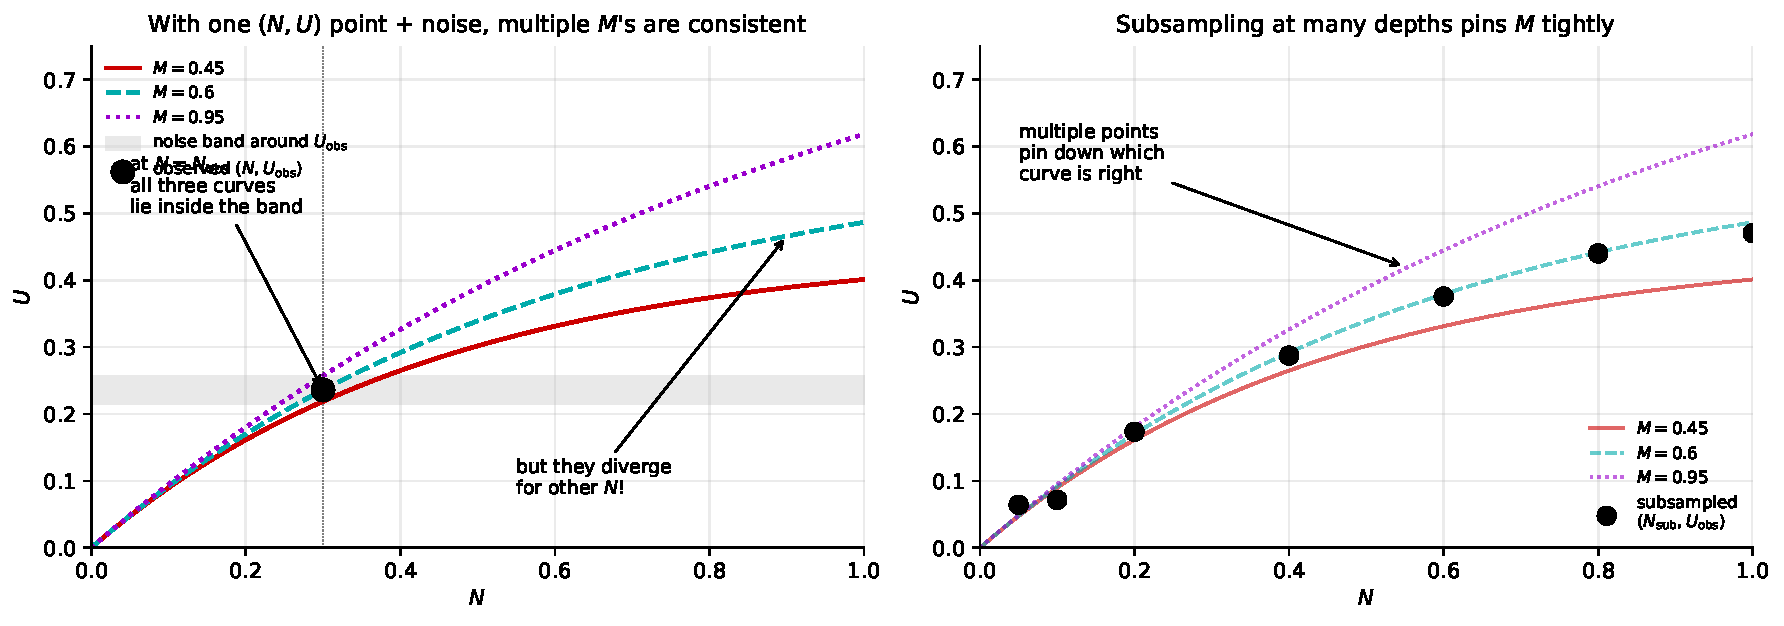
\includegraphics[width=0.8\linewidth]{fig2_ambiguity.pdf}
\caption{Three saturation curves with different $M$ all pass near a single observed
$(N, U)$. One point alone doesn't tell you which $M$ generated the data.}
\label{fig:ambig}
\end{figure}

This is the lecture's warning: \emph{``a single $(N, U)$ pair pins $M$ down only
weakly''}. The fix is to give the estimator multiple anchor points -- which is exactly
what subsampling does.

\section{The subsampling protocol}

We have one dataset at depth $N$. We \emph{pretend} we'd sequenced less, by randomly
discarding most of the reads. For a depth fraction $d \in (0, 1]$ we keep
$\Nsub = \lfloor dN \rfloor$ reads chosen uniformly at random without replacement,
then count how many distinct fragments survived; call that $\Uobs(\Nsub)$.

Doing this at several depths gives us a curve of empirical points
$(\Nsub^{(1)}, \Uobs^{(1)}), \dots, (\Nsub^{(K)}, \Uobs^{(K)})$ that should trace the
saturation curve. A standard depth grid is
\[
   d \in \{0.05,\; 0.1,\; 0.2,\; 0.4,\; 0.6,\; 0.8,\; 1.0\}.
\]

\begin{figure}[h]
\centering
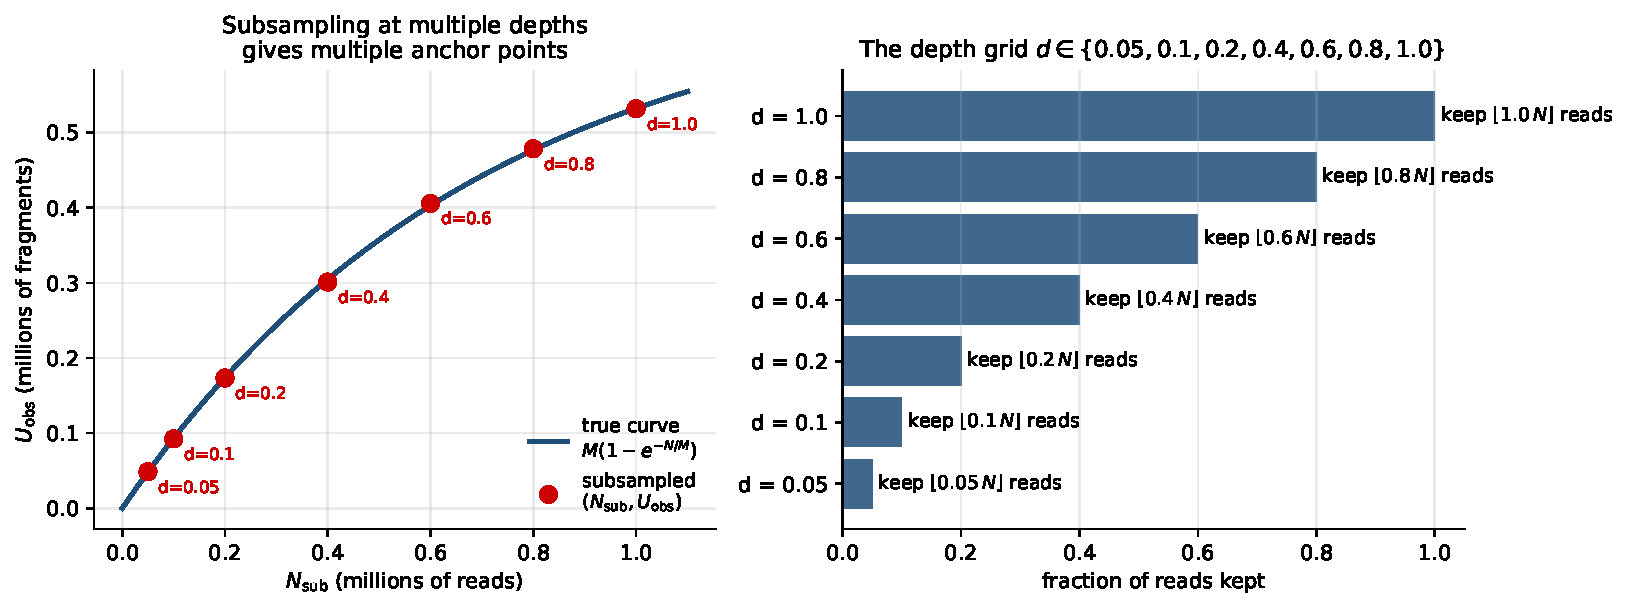
\includegraphics[width=\linewidth]{fig3_subsampling.pdf}
\caption{Subsampling protocol. Left: each depth fraction $d$ gives one
$(\Nsub, \Uobs)$ point; together they trace the saturation curve. Right: the depth
grid -- at $d = 0.05$ we keep 5\% of the reads; at $d = 1.0$ we use everything.}
\label{fig:subs}
\end{figure}

\paragraph{How to do the subsampling concretely.}
Two equivalent options, take whichever you prefer:

\begin{tcolorbox}[breakable,colback=blue!4,colframe=blue!55!black,title=\textbf{Option A: random subsampling (Monte Carlo)}]
The idea: simulate ``what would have happened if the sequencer had stopped after only
$\Nsub$ reads.''

\textbf{The trick is to picture the data as a bag of $N$ reads.} Our file gives us
fragments and per-fragment counts, but each row really represents several reads of the
same fragment. So we mentally (or actually, in code) flatten the file into a single
list of $N$ tickets, one per read, each ticket labelled with the index of its parent
fragment.

\emph{Tiny example.} Three fragments with counts $(n_1, n_2, n_3) = (3, 1, 2)$ give
$N = 6$ reads, and the flat list is
\[
   \underbrace{[\,1,\;1,\;1,\;2,\;3,\;3\,]}_{\text{6 tickets}}.
\]
Fragment $1$ has 3 tickets in the bag, fragment $2$ has 1, fragment $3$ has 2. Drawing
$\Nsub = 3$ tickets at random without replacement might yield $[1, 3, 2]$ -- three
distinct fragments observed, so $\Uobs = 3$ -- or $[1, 1, 3]$ -- two distinct fragments,
$\Uobs = 2$. The randomness comes from which $\Nsub$ tickets we pulled.

\textbf{In code, for each depth fraction $d$:}
\begin{enumerate}[leftmargin=2em,itemsep=2pt]
  \item Build the flat ticket array of length $N$: \texttt{np.repeat(np.arange(U), n)}
        creates the list above for any count array \texttt{n}.
  \item Pick $\Nsub = \lfloor dN \rfloor$ tickets at random without replacement
        (\texttt{rng.choice(tickets, size=Nsub, replace=False)}).
  \item Count the number of distinct ticket labels in your pick. That is the empirical
        $\Uobs(\Nsub)$.
\end{enumerate}
Repeat across a few random seeds and average if you want a smoother curve.
\end{tcolorbox}

\begin{tcolorbox}[breakable,colback=blue!4,colframe=blue!55!black,title=\textbf{Option B: Heck's rarefaction (the same thing, but in closed form)}]
Option~A is randomised: every time you re-run it you get a slightly different $\Uobs$.
It turns out we can write down the \emph{expected} $\Uobs$ -- averaged over all possible
random draws -- in closed form, so we don't need to sample at all.

\textbf{Setup.} We pick $s$ tickets out of $N$ uniformly at random without replacement.
Fragment $j$ owns $n_j$ of those tickets. We want the probability that we observe
fragment $j$ at least once, i.e.\ at least one of $j$'s $n_j$ tickets ends up in our
$s$-pick.

\textbf{Easier to compute the complement -- the probability we \emph{miss} $j$.} We
miss $j$ iff all $s$ tickets we picked are from the $N - n_j$ ``not-$j$'' tickets.
Counting:
\begin{align*}
   \#\{\text{ways to pick } s \text{ tickets, none of which are } j\}
       &\;=\; \binom{N - n_j}{s}, \\
   \#\{\text{ways to pick any } s \text{ tickets}\}
       &\;=\; \binom{N}{s},
\end{align*}
so $\Pr(\text{miss } j) = \dbinom{N - n_j}{s} \big/ \dbinom{N}{s}$, and consequently
\begin{equation}
   \E\bigl[\Uobs(s)\bigr]
   \;=\; \sum_{j=1}^{U} \Pr(\text{observe } j)
   \;=\; \sum_{j=1}^{U} \!\Biggl[\, 1 - \frac{\binom{N - n_j}{s}}{\binom{N}{s}} \,\Biggr].
   \label{eq:heck}
\end{equation}
This is \textbf{Heck's rarefaction formula}: the exact expected number of distinct
fragments at sample size $s$, given the per-fragment counts $n_j$ we already have.

\textbf{Why log-space.} For $N = 4{,}000{,}000$ and $s = 2{,}000{,}000$, $\binom{N}{s}$
is astronomically large -- no floating-point format can hold it. The workaround is to
use $\log \binom{N}{s} = \log\Gamma(N+1) - \log\Gamma(s+1) - \log\Gamma(N - s + 1)$
(computed by \texttt{scipy.special.gammaln}, which returns $\log\Gamma$). Take the
difference of two such logs to get a manageable number $-c$, exponentiate
($e^{-c}$, the miss probability), and only \emph{then} subtract from $1$ and sum. No
overflow, no random seed, just one pass over the $n_j$ values per $s$.
\end{tcolorbox}

\textbf{The two options are the same algorithm,} one randomised and one in closed form.
For the homework either is fine -- Option~A is more intuitive (you actually simulate
the subsampling), Option~B is faster and deterministic (no seed to fix, no Monte Carlo
noise). They agree because Equation~\eqref{eq:heck} is precisely $\E[\Uobs]$ averaged
over the randomness of Option~A.

\section{Fitting $M$ to the empirical curve}

Now we have $K$ pairs $(\Nsub^{(i)}, \Uobs^{(i)})$. We choose $M$ to minimise the sum
of squared residuals against the saturation curve:
\begin{equation}
   \hM \;=\; \arg\min_{M > 0}\; \sum_{i=1}^{K} \Bigl(\, \Uobs^{(i)} - M\bigl(1 - e^{-\Nsub^{(i)}/M}\bigr) \,\Bigr)^2.
   \label{eq:fit}
\end{equation}

In Python this is a one-liner with \texttt{scipy.optimize.curve\_fit}:
\begin{quote}\small
\texttt{def model(N, M): return M * (1 - np.exp(-N/M))} \\
\texttt{M\_hat, \_ = curve\_fit(model, N\_subs, U\_obs, p0=[max(U\_obs)*2])}
\end{quote}

The initial guess $p_0$ matters only because $M$ appears non-linearly: any $M$ bigger
than the largest observed $\Uobs$ is a safe starting point (since $\E[U] < M$ always).

\begin{figure}[h]
\centering
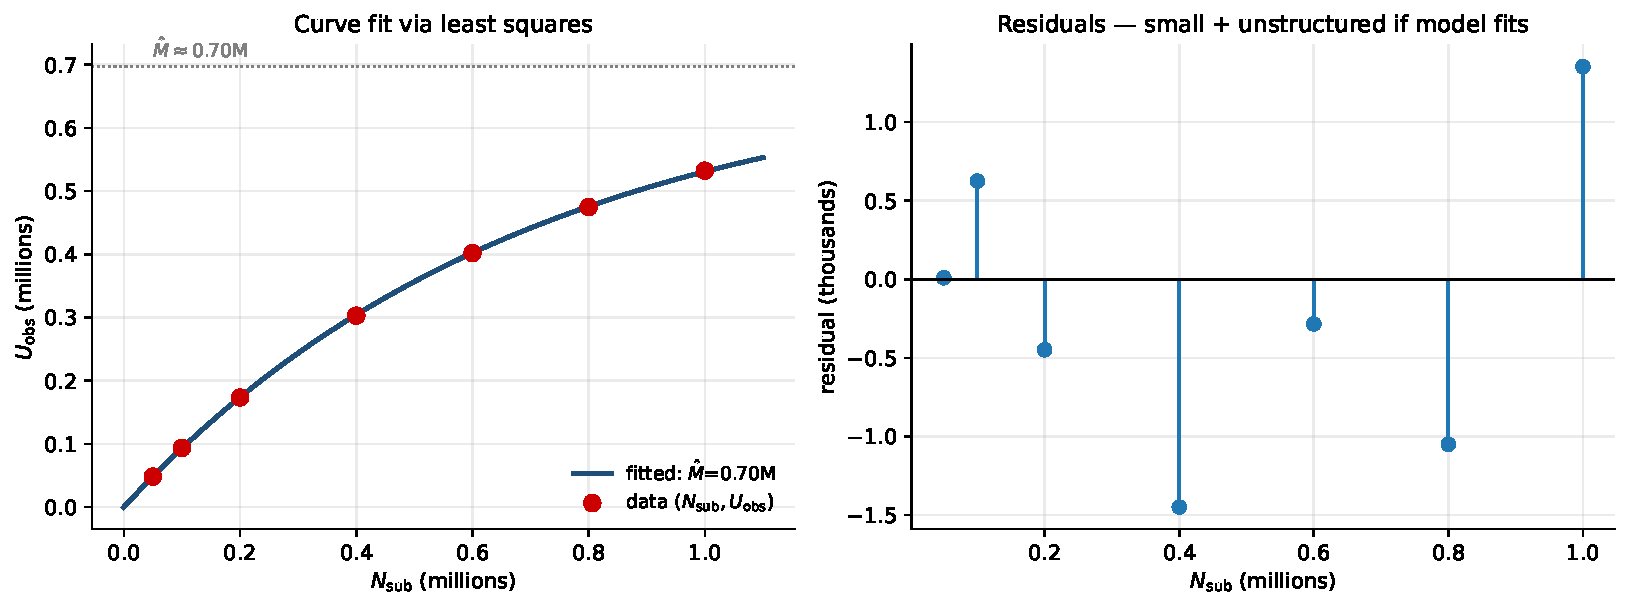
\includegraphics[width=\linewidth]{fig4_fit.pdf}
\caption{Left: simulated $(\Nsub, \Uobs)$ points (red) overlaid on the fitted curve
$\hM(1-e^{-N/\hM})$ (blue). The dotted line marks the asymptote $\hM$. Right:
residuals; if the saturation model fits, they are small and unstructured.}
\label{fig:fit}
\end{figure}

\section{What the curve fit tells you that the single-point estimator does not}

By Q1(c), the single-equation Setup/MLE estimator solves
$\lambda/(1 - e^{-\lambda}) = N/U$, an algebraic identity using only the endpoint
$(N, U)$. It throws away the rest of the saturation curve. The subsampling fit uses the
whole curve, so it is sensitive to \emph{the shape}, not just the endpoint:

\begin{itemize}[leftmargin=2em,itemsep=2pt]
  \item \textbf{If the data really follow $M(1-e^{-N/M})$,} the two estimators give the
        same answer up to noise.
  \item \textbf{If they disagree,} the data is telling you the uniform-$\lambda$ model
        is wrong. The MLE forces the model through the endpoint; the curve fit averages
        across depths, and the difference between them is a diagnostic of
        misspecification. (Q3 will study exactly such misspecification, with
        fragment-length-dependent $\lambda$.)
\end{itemize}

\section{Implementation outline}

A clean Q2(a) script looks like:

\begin{tcolorbox}[colback=gray!8,colframe=gray!50,title=\textbf{Pseudocode}]
\small
\begin{verbatim}
for each file:
    read (chr, start, end, n) rows
    N = sum(n);   U = number of rows
    # --- MLE branch ---
    lam_hat_MLE = brentq(lambda L: L/(1-exp(-L)) - N/U,  1e-10,  N/U)
    M_hat_MLE  = N / lam_hat_MLE
    # --- subsampling branch (Heck) ---
    depths = [0.05, 0.1, 0.2, 0.4, 0.6, 0.8, 1.0]
    N_subs = [floor(d*N) for d in depths]
    U_subs = [heck_expected_U(n_array, s) for s in N_subs]
    M_hat_fit, _ = curve_fit(model, N_subs, U_subs, p0=[max(U_subs)*2])
    report (file, N, U, M_hat_MLE, M_hat_fit, M_hat_fit/M_hat_MLE)
\end{verbatim}
\end{tcolorbox}


\end{document}
